\subsection{Información personal}

  \subsubsection{Establecer curso académico}

  \paragraph{}La aplicación permite establecer el curso académico para el que
  el usuario puede gestionar su información. Esto permite ver la información
  guardada en cursos académicos pasados, permitiendo la posibilidad de cambiar
  dicha información, en el caso de que fuera errónea.

  \paragraph{}Para establecer el curso académico en el que se realizará la labor
  de asesoría, es necesario pulsar en el icono \textit{Curso académico}, el cual
  está situado en el menú de sesión descrito en el capítulo
  \ref{gestionInformacion}, \textit{Gestión de la información}. Se puede ver una
  captura de pantalla de este icono en la figura
  \ref{capturaPantallaIconoCursoAcademico}.

  \begin{figure}[!ht]
    \begin{center}
      \fbox{
      
\includegraphics[scale=0.55]{4.Funcionamiento_Aplicacion/4.3.Gestion/4.3.3.Asesor/4.3.3.9.InformacionPersonal/icono_curso_academico.png}
      }
      \caption{Captura de pantalla del icono \textit{Curso académico}.}
      \label{capturaPantallaIconoCursoAcademico}
    \end{center}
  \end{figure}

  \paragraph{}Una vez pulsado el icono, la aplicación nos llevará a un
  formulario para que introduzcamos el curso académico que queremos establecer.
  Este formulario es el mostrado por la figura
  \ref{capturaPantallaSetCursoAcademico}. Si el curso académico es válido para
  el usuario que está utilizando la aplicación, se hará efectivo el cambio de
  curso académico. En caso contrario se mostrará un mensaje de error.

  \begin{figure}[!ht]
    \begin{center}
      \fbox{
      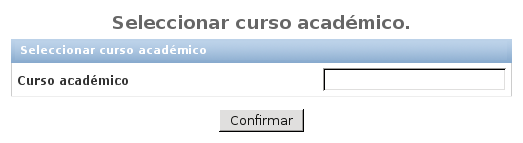
\includegraphics[scale=0.55]{4.Funcionamiento_Aplicacion/4.3.Gestion/4.3.3.Asesor/4.3.3.9.InformacionPersonal/set_curso_academico.png}
      }
      \caption{Captura de pantalla del formulario de selección de \textit{Curso académico}.}
      \label{capturaPantallaSetCursoAcademico}
    \end{center}
  \end{figure}

  \subsubsection{Ver información personal}

  \paragraph{}Este usuario tendrá la posibilidad de ver y editar la información
  personal que está albergada en el sistema. Esta operación se realiza mediante
  el formulario de edición de información personal, el cual se muestra en la
  figura \ref{capturaModificarDatosAsesor}.

  \begin{figure}[!ht]
    \begin{center}
      \fbox{
      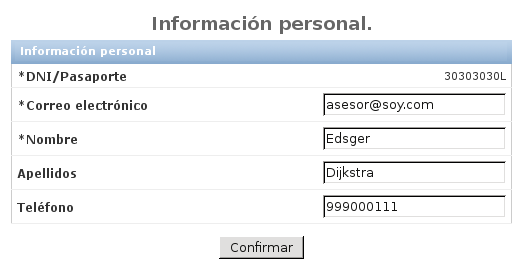
\includegraphics[scale=0.55]{4.Funcionamiento_Aplicacion/4.3.Gestion/4.3.3.Asesor/4.3.3.9.InformacionPersonal/edit_datos_asesor.png}
      }
      \caption{Captura de pantalla del formulario de edición de datos personales para el usuario \textit{Asesor}.}
      \label{capturaModificarDatosAsesor}
    \end{center}
  \end{figure}


  \subsubsection{Modificar contraseña}

  \paragraph{}Para este usuario, estará disponible la posibilidad de cambiar su
  contraseña en el sistema. Para llevar a cabo esta operación, deberá seguir los
  mismos pasos indicados en la sección \ref{modificarPassword}.

  \paragraph{}Una vez rellenado el formulario, se pulsará el botón
  \textit{Confirmar}, el cual se puede ver en la figura
  \ref{capturaBotonConfirmar}. Si el formulario rellenado es válido, y no tiene
  errores, se editará la información personal en el sistema. En caso de
  contener información no válida, un mensaje de error aparecerá indicando los
  campos del formulario que no han pasado la validación, los cuales habrá que
  modificar para modificar correctamente los datos personales en el sistema.
